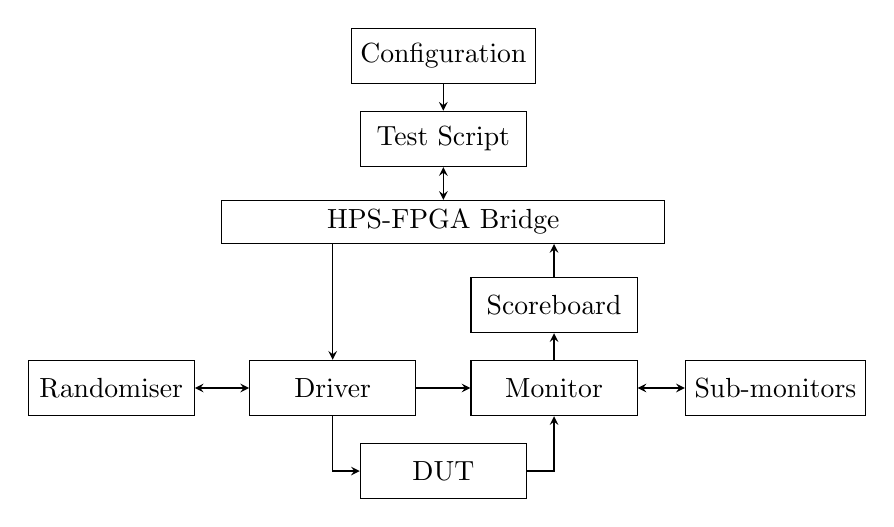
\begin{tikzpicture}
  [
    x=1em, y=1em,
    block/.style =
      {draw, rectangle, align=center, minimum width=6em, minimum height=2em},
    inter/.style =
      {draw, rectangle, align=center, minimum width=16em, minimum height=1em}
  ]
  \node [block] at (-8,3)  (r) {Randomiser};
  \node [block] at ( 0,3)  (d) {Driver};
  \node [block] at ( 4,0)  (t) {DUT};
  \node [block] at ( 8,6)  (s) {Scoreboard};
  \node [block] at ( 8,3)  (m) {Monitor};
  \node [block] at (16,3)  (u) {Sub-monitors};
  \node [inter] at ( 4,9)  (b) {HPS-FPGA Bridge};
  \node [block] at ( 4,12) (w) {Test Script};
  \node [block] at ( 4,15) (f) {Configuration};

  \draw[<->, >=stealth] (r.east)           -- (d.west);
  \draw[ ->, >=stealth] (d.south)          |- (t.west);
  \draw[ ->, >=stealth] (t.east)           -| (m.south);
  \draw[ ->, >=stealth] (m.north)          -- (s.south);
  \draw[ ->, >=stealth] (b.south-|d.north) -- (d.north);
  \draw[ ->, >=stealth] (s.north)          -- (b.south-|s.north);
  \draw[<->, >=stealth] (b.north)          -- (w.south);
  \draw[ ->, >=stealth] (f.south)          -- (w.north);
  \draw[ ->, >=stealth] (d.east)           -- (m.west);
  \draw[<->, >=stealth] (m.east)           -- (u.west);
\end{tikzpicture}